\chapter{Modification of Optical Properties – Controlling Laser Light}
\section{Introduction}
Une bonne question d'examen est \textit{comment changer la polarisation}. On peut parler des matériau
non-isotrope, surface normal, index ellipsoid, \dots\ Une autre bonne question d'examen est 
\textit{Comment modifier une mode}, et ça, c'est l'objectif de ce chapitre. Si on s'intéresse à la
modification d'onde, c'est pour y placer des informations. \\

Nous allons ainsi considérer ici l'effet d'un champ appliqué (magnétique ou électrique) sur la propagation 
d'ondes électromagnétiques dans les cristaux. Dans certains cristaux, la présence d'un champ appliqué va
modifier son index ellipsoid et donc ses modes propres. 

\section{Electro-Optics}
\subsection{Microscopic Theory}
Ce domaine n'existe que depuis une soixantaine d'années car il a fallu attendre l'invention du laser, 
permettant l'obtention de grande puissance optique. Cette grande puissance permettra l'intervention des
ions. On assumera dans ce chapitre que $\vec{\epsilon}$ est modulé à basse fréquence, bien plus petite que celle
de la porteuse, afin de mettre ces ions en mouvement. \\

La susceptibilité dépend des charges liées et de la force avec lesquelles ces électrons sont liés au
noyau. Lorsqu'on applique un champ électrique $\vec{\epsilon}$, les charges liées sont redistribuées et
le réseau ionique est légèrement déformé : le tenseur d'imperméabilité est modifié et, par conséquent, 
les dimension et l'orientation de l'index ellipsoid est modifiée. C'est l'effet \textbf{électro-otpique}. Si
$\vec{\epsilon}$ est petit, on peut développer en série l'imperméabilité
\begin{equation}
\bar{\bar{\eta}}(\epsilon) = \bar{\bar{\eta}}^{(0)}+\bar{\bar{\bar{r}}}.\epsilon + \bar{\bar{\bar{\bar{s}}}}:
\epsilon\epsilon
\end{equation}
En notation indicielle
\begin{equation}
\eta_{ij}(\epsilon) = \eta_{ij}^{(0)}+r_{ijk}\epsilon_k+s_{ijkl}\epsilon_k\epsilon_l
\end{equation}
où $\eta_{ij}^{(0)}$ est le tenseur non perturbé donné par
\begin{equation}
\bar{\bar{\eta}} = \left(\begin{array}{ccc}
\frac{1}{n^2_1}&0&0\\
0&\frac{1}{n^2_2}&0\\
0&0&\frac{1}{n^2_3}
\end{array}\right)
\end{equation}
où les constantes $r_{ijk}$ sont les \textbf{coefficients de Pockels}, décrivant les effets électro-optiques
linéaires ($\approx 10^{-12}$ m.V$^{-1}$). Souvent, ces coefficients sont nuls (si le matériau possède une
centrosymétrie) et le second terme devient dominant.Les constants $s_{ijklm}$ sont les \textbf{coefficients
de Kerr}, décrivant les effets électro-optique quadratiques ($\approx 10^{-15}$ m$^2$.V$^{-2}$). \\

Comme les effets électro-optiques sont liés au mouvement ionique, les coefficients sont indépendants de la
fréquence si le voltage est tel que l'on se situe loin des résonances ioniques. On peut alors considérer
les coefficients de Pockels et Kerr comme \textbf{statiques}.

\subsection{Symmetry Properties of Pockels’ Tensor}
\subsubsection{Kleinmann Convention}
Si le milieu est sans pertes et sans activité optique, son tenseur diélectrique est symétrique. Par 
définition, le tenseur d'imperméabilité doit également l’être dans ces conditions. On en déduit que
le tenseur de Pockels est \textit{invariant} pour une permutation de $i$ et $j$ : on passe de 27 à 
18 composants indépendants ! Pour se simplifier la vie, on va "tabuler" le tenseur d'imperméabilité 
de l'effet Pockels et Kerr selon la \textbf{convention de Kleinmann}
\begin{equation}
\begin{array}{lll}
1&=(11)\\
2&=(22)\\
3&=(33)\\
4&=(23)&=(32)\\
5&=(31)&=(13)\\
6&=(12)&=(21)
\end{array}
\end{equation}
Selon cette convention, on peut \textbf{représenter} le tenseur de Pockels comme un tableau $6\times 3$ 
mais attention ce n'est \textbf{pas} un tenseur (pas question de lui appliquer les propriétés des teneurs)
\begin{equation}
\left(\begin{array}{ccc}
r_{11} = r_{111} & r_{12} = r_{112} & r_{13} = r_{113}\\
r_{21} = r_{221} & r_{22} = r_{222} & r_{23} = r_{223}\\
r_{31} = r_{331} & r_{32} = r_{332} & r_{33} = r_{333}\\
r_{41} = r_{231} & r_{42} = r_{232} & r_{43} = r_{233}\\
r_{51} = r_{311} & r_{52} = r_{312} & r_{53} = r_{313}\\
r_{61} = r_{121} & r_{62} = r_{122} & r_{63} = r_{123}
\end{array}\right)
\end{equation}

\newpage
\subsubsection{Principe de Neumann}
On peut encore réduire le nombre de composants indépendants du tenseur de Pockels à l'aide du 
principe de Neumann :
\begin{center}
\textit{Les éléments de symétrie de tout tenseur associé à une propriété matérielle d'un cristal doivent inclure toutes les propriétés de symétrie du groupe de points du cristal.}
\end{center}
Si ce principe est d'application, on en tire que
\begin{equation}
r_{ijk}' = r_{ijk}
\end{equation}
Ce principe démontre la non-présence de l'effet Pockels pour les matériaux centro-symétriques. L'inversion
spatiale pour un tenseur du troisième rang s'écrit 
\begin{equation}
r_{ijk}' = -r_{ijk}
\end{equation}
Selon le principe de Neumann ($r_{ijk}' = r_{ijk}$), on en tire
\begin{equation}
r_{ijk}=0
\end{equation}

\subsection{The Linear Electro-Optic Effect}
Soit un cristal couplé lelong de ses axes principaux sur lequel est appliqué un champ électrique. Une
onde EM incidente va "voir" l'anisotropy et les effets dus au champ électrique. On s'intéresse ici à 
ce qui va se passer dans l'onde qui se propage dans le cristal. \\

Pour trouver les propriétés de propagation d'une onde plane monochromatique, il faut connaître le
tenseur d'imperméabilité : on pourra en déduire le système de coordonnée principal et trouver les 
indices principaux (voir \textit{chapitre 1}). Supposons que le tenseur de Pockels soit non-nul : 
on peut négliger les effets quadratiques :
\begin{equation}
\eta_{ij}(\epsilon) = \eta_{ij}^{(0)}+r_{ijk}\epsilon_k
\end{equation}
Il y a beaucoup de termes la dedans. En utilisant cette expression, on peut trouver l'index ellipsoid
\begin{equation}
\left(\dfrac{1}{n^2_1}+r_{1k}\epsilon_{1k}\right)X^2+
\left(\dfrac{1}{n^2_2}+r_{1k}\epsilon_{2k}\right)Y^2+
\left(\dfrac{1}{n^2_3}+r_{1k}\epsilon_{3k}\right)Z^2+ 
2r_{4k}\epsilon_kYZ + 2r_{5k}\epsilon_kZX+2r_{6k}\epsilon_kXY=1
\label{eq:6.11}
\end{equation}
où $1/n_i^2$ sont les valeurs propres du tenseur d'imperméabilité non-perturbé et $\epsilon_k$ les composantes
du champ électrique appliqué (quand $\epsilon_k=0$, on retrouve l'ellipse non-perturbé). On voit apparaître
trois nouveaux termes non-diagonaux : les axes principaux de l'index ellipsoid perturbés ne coïncident pas avec
ceux de la non-perturbée : elle a subit une rotation. Par rotation, on peut donc retrouver les nouveaux axes
principaux. 

\newpage
\exemple{Considérons l'effet électro-optique dans le KDP. Il s'agit d'un cristal $\bar{42}m$ : axe de 
symétrie incorrect quadruple (rotation de $\pi/2$ autour de l'axe suivi d'une réflexion sur un plan
perpendiculaire à l'axe), conventuellement considéré comme l'axe $z$.  On trouve comme tenseur
\begin{equation}
\left(\begin{array}{ccc}
0&0&0\\
0&0&0\\
0&0&0\\
r_{41}&0&0\\
0&r_{41}&0\\
0&0&r_{63}
\end{array}\right)
\end{equation}
où seuls trois coefficient de Pockels sont non-nuls. L'index ellipsoid devient alors
\begin{equation}
\dfrac{1}{n_0^2}X^2+\dfrac{1}{n_0^2}Y^2+\dfrac{1}{n_0^2}Z^2 + 2r_{41}\epsilon_xYZ+2r_{41}\epsilon_y
ZX+2r_{63}\epsilon_zXY=1
\label{eq:6.13}
\end{equation}
	\begin{center}
	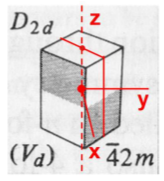
\includegraphics[scale=0.5]{ch6/image1}
	\captionof{figure}{Groupe de symétrie pour le KDP}
	\end{center}

}


\subsubsection{Effet Pockels longitudinal}
Il s'agit du cas où le champ appliqué est parallèle à l'axe de symétrie du cristal
\begin{equation}
\vec\epsilon=\epsilon\vec{1}_z
\end{equation}
L'équation \eqref{eq:6.13} devient
\begin{equation}
\dfrac{X^2+Y^2}{n_0^2}+\dfrac{Z^2}{n_e^2}+2r_{63}\epsilon XY=1
\label{eq:6.15}
\end{equation}
où le dernier terme est \textit{mixte}. Pour étudier les effets, il faut connaître les axes principaux
et les nouveaux indices de réfraction. Pour obtenir la forme standard (sans termes mixtes), il faut effectuer 
une rotation du système autour de l'axe $z$.\\

	\begin{wrapfigure}[6]{l}{5cm}
	\vspace{-5mm}
	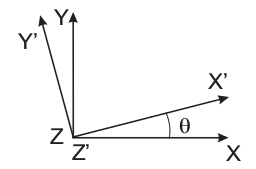
\includegraphics[scale=0.5]{ch6/image2}
	\captionof{figure}{ }
	\end{wrapfigure}
La transformation et son la transformation inverse associée sont données par
\begin{equation}
\left\{\begin{array}{lll}
X' &= X\cos\theta &+ Y\sin\theta\\
Y' &= -X\sin\theta&+ Y\cos\theta\\
Z' &= Z
\end{array}\right.\qquad\qquad
\left\{\begin{array}{lll}
X &= X'\cos\theta &- Y'\sin\theta\\
Y &= X'\sin\theta&+ Y'\cos\theta\\
Z &= Z'
\end{array}\right.
\end{equation}
La substitution dans \eqref{eq:6.15} donne
\begin{equation}
\left(\dfrac{1}{n_0^2}+2r_{63}\epsilon\sin\theta\cos\theta\right)X^{'2}+
\left(\dfrac{1}{n_0^2}-2r_{63}\epsilon\sin\theta\cos\theta\right)Y^{'2}+\dfrac{1}{n_e^2}Z^{'2}+
2r_{63}\epsilon(\cos^2\theta-\sin^2\theta)X'Y'=1
\label{eq:6.18}
\end{equation}
Le terme mixte disparaît si
\begin{equation}
2r_{63}\epsilon(\cos^2\theta-\sin^2\theta)=0\quad\Leftrightarrow\quad \tan\theta=1\quad
\Leftrightarrow\quad\theta=\pm\frac{\pi}{4}
\end{equation}

	\begin{wrapfigure}[12]{r}{4cm}
%	\vspace{-5mm}
	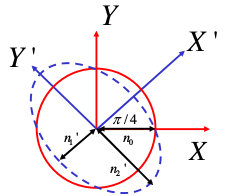
\includegraphics[scale=0.5]{ch6/image3}
	\captionof{figure}{ }
	\end{wrapfigure}
Sous l'application d'un champ électrique, l'index ellipsoid est donc \textbf{tournée de 45$^\circ$} 
par rapport au cas où $\vec{\epsilon}=\vec0$. On peut obtenir les nouveaux indices de réfraction à partir de
\eqref{eq:6.18}
\begin{equation}
n_1' = \left(\dfrac{1}{n_o^2}+r_{63}\epsilon\right)^{-\frac{1}{2}} \approx n_o-\frac{1}{2}n_o^3r_{63}\epsilon
\label{eq:6.20}
\end{equation}
\begin{equation}
n_1' = \left(\dfrac{1}{n_o^2}-r_{63}\epsilon\right)^{-\frac{1}{2}} \approx n_o+\frac{1}{2}n_o^3r_{63}\epsilon
\end{equation}
\begin{equation}
n_3'=n_3=n_e
\end{equation}
La variation des deux indices principaux est proportionnelle aux coefficients de Pockels et au cube de
l'indice ordinaire non-perturbé.



\subsubsection{Effet Pockels transverse}
Considérons cette fois-ci le même cristal KDP (point group $\bar{42}m$) mais avec un champ électrique
appliqué parallèle à l'axe $y$. L'équation \eqref{eq:6.11} devient maintenant
\begin{equation}
\dfrac{X^2+Y^2}{n_o^2}+\dfrac{Z^2}{n_e^2}+2r_{41}\epsilon XZ = 1
\label{eq:6.21}
\end{equation}
Il n'y a ici qu'un terme \textit{mixte} entre $X$ et $Z$ : $y$ reste un axe principal du système et une
rotation autour de cet axe est nécessaire pour retrouver la forme standard de l'index ellipsoid.
\begin{equation}
\left\{\begin{array}{lll}
X&=Z'\sin\theta&+X'\cos\theta\\
Y&=Y'\\
Z&=Z'\cos\theta&-X'\sin\theta
\end{array}\right.
\label{eq:6.22}
\end{equation}
La substitution de \eqref{eq:6.22} dans \eqref{eq:6.21} donne
\begin{equation}
\begin{array}{ll}
&\phantom{+}\DS X^{'2}\left(\dfrac{\cos^2\theta}{n_o^2}+\dfrac{\sin^2\theta}{n_e^2}-r_{41}\epsilon\sin2\theta\right)\vspace{2mm}\\
&+\DS Y^{'2}\left(\dfrac{\sin^2\theta}{n_o^2}+\dfrac{\cos^2\theta}{n_e^2}-r_{41}\epsilon\sin2\theta\right)\vspace{2mm}\\
&+\DS Y^{'2}\left(\dfrac{1}{n_o^2}\right)\vspace{2mm}\\
&+\DS Z'X'\left[\sin2\theta\left(\dfrac{1}{n_o^2}-\dfrac{1}{n_e^2}\right)+2r_{41}\epsilon\left(\cos^2\theta
-\sin^2\theta\right)\right]=1
\end{array}
\end{equation}
Pour faire disparaître le terme mixte, il faut que
\begin{equation}
\tan2\theta=-\dfrac{2r_{41}\epsilon}{\dfrac{1}{n_o^2}-\dfrac{1}{n_e^2}}\qquad\Leftrightarrow\qquad
\theta\approx -\dfrac{r_{41}\epsilon}{\dfrac{1}{n_o^2}-\dfrac{1}{n_e^2}}
\end{equation}
où l'approximation est possible, le coefficient de Pockels étant petit devant 1 et le champ électrique
appliqué est limité pour éviter le claquage. Après quelques manipulations trigonométriques (sans 
approximation)
\begin{equation}
X^{'2}\left(\dfrac{1}{n_o^2}-r_{41}\epsilon\tan\theta\right)+
Z^{'2}\left(\dfrac{1}{n_o^2}+r_{41}\epsilon\tan\theta\right)+
Y^{'2}\left(\dfrac{1}{n_o^2}\right)=1
\end{equation}
On peut en déduire les indices de réfraction. Pour le premier
\begin{equation}
n_1' =\left(\dfrac{1}{n_o^2}-r_{41}\epsilon\tan\theta\right)^{-\frac{1}{2}}\approx
n_o+\frac{1}{2}n_o^3r_{41}\epsilon.\theta
\end{equation}
Comme $\theta\propto \epsilon\to n_i' \propto \epsilon^2$ ce qui n'est pas très pratique : on n'utilise
pas l'effet Pockels transverse en pratique. De plus, on ne peut utiliser cette approche pour le KDP à 
cause de cette dépendance en $\epsilon^2$ : on ne peut pas négliger les effets NL quadratiques.


\subsection{Polarisation, Amplitude and Phase Modulation}
L'effet Pockels longitudinal permet de modifier la polarisation en $y$. Il est possible de moduler un
signal en appliquant un champ électrique. L'application de celui-ci va faire tourner l'index ellipsoid
de 45$^\circ$. Le champ incident va être projeté dans les nouveaux axes, de façon équitable. Comme
les deux axes sont différents, on va pouvoir induire des retards. 

\subsubsection{Polarisation modulation}
Soit un cristal KDP, un champ appliqué parallèle à $z$ et une onde plane monochromatique polarisée
linéairement selon l'axe $y$ (non-perturbé) se propageant en $z$, incident sur le celui-ci\footnote{Par
exemple avec un polariseur juste avant le cristal}
\begin{equation}
\vec E = E_0e^{i(\omega t-kz))}\vec{1_y}
\end{equation}
Lorsque aucun champ n'est appliqué, cette onde est un mode propre de propagation et il va se propager
sans voir sa polarisation modifiée. Avec un champ électrique appliqué ce n'est plus le cas, mais une 
superposition de deux modes d'indices $n_1'$ et $n_2'$ superposés, donné par \eqref{eq:6.20} \& al. 
\begin{equation}
E(z,t) = \dfrac{E_0}{\sqrt{2}}e^{i\left(\omega t-\frac{\omega}{c}n_1'z\right)}\vec{1_x}+
\dfrac{E_0}{\sqrt{2}}e^{i\left(\omega t-\frac{\omega}{c}n_2'z\right)}\vec{1_y}
\end{equation}
Pour un cristal d'épaisseur $L$, le retard de phase est donné par
\begin{equation}
\begin{array}{ll}
\Gamma &\DS= \left(\omega-\dfrac{\omega}{c}n_1'L\right)-\left(\omega-\dfrac{\omega}{c}n_2'L\right)\vspace{2mm}\\
&\DS=-\dfrac{\omega}{c}L\left(n_o-\dfrac{1}{2}n_o^3r_{63}\epsilon\right)+\dfrac{\omega}{c}L\left(n_o+\dfrac{1}{2}n_o^3r_{63}\epsilon\right)\vspace{2mm}\\
&=\DS\dfrac{\omega}{c}n_o^3r_{63}V = \dfrac{2\pi}{\lambda_0}n_o^3r_{63}V
\end{array}
\end{equation}
Le retard de phase est directement proportionnel à la tension appliquée et donc proportionnel à $\epsilon$. 
Si $\Gamma=\pi$, le rayon qui quitte le cristal est toujours polarisé linéairement, mais tourne de 
$90^\circ$. La tension correspondant à ceci est de
\begin{equation}
V_{pi} = \dfrac{\lambda_0}{2n_o^3r_{63}}
\end{equation}
Celle-ci permet la modulation. Pour un KDP avec $\lambda=632.8$nm, elle vaut $8.4$ kV.


\subsection{Modulation en amplitude}
On peut utiliser le même dispositif en plaçant à la fin un analyseur placé orthogonalement au polariseur
d'entrée
\begin{center}
	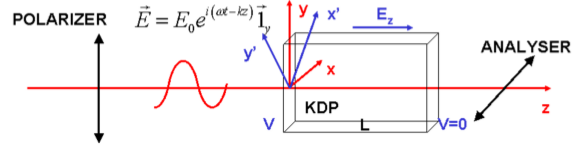
\includegraphics[scale=0.5]{ch6/image4}
	\captionof{figure}{Modulation en amplitude}
\end{center}
La \textit{page 102} reprend le développement de l'onde en sortie, à l'aide des matrices de 
\textsc{Jones} (champ d'entrée, rotation, propagation dans les axes, rotation inverse). On trouve la
même expression de $\Gamma$ que précédemment et comme champ en sortie
\begin{equation}
E_{out} = E_{in}\sin\dfrac{\Gamma}{2}\vec{1_x}
\end{equation}
Il est plus pratique de travailler en intensité
\begin{equation}
I_{out} = \frac{1}{2}\epsilon_0c|E_{out}|^2 = \frac{1}{2}\epsilon_0c E_{in}^2\sin^2\frac{\Gamma}{2}
\end{equation}

	\begin{wrapfigure}[12]{r}{7cm}
	\vspace{-5mm}
	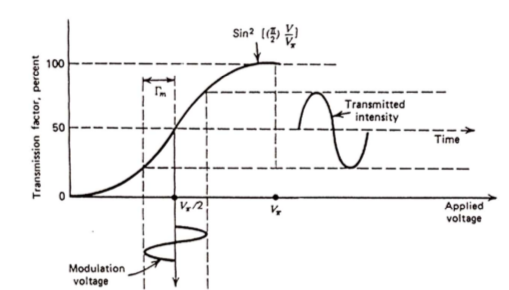
\includegraphics[scale=0.4]{ch6/image5}
	\captionof{figure}{ }
	\end{wrapfigure}
La transmission (représentée ci-contre) est donnée par
\begin{equation}
T \equiv \dfrac{I_{out}}{I_{in}} = \sin^2\left(\dfrac{\pi}{2}\dfrac{V}{V_\pi}\right)
\end{equation}
A cause de la non-linéarité de cette courbe, de nouvelles harmoniques peuvent être créées. Pour 
limiter celles-ci, on va travailler proche du point d’inflexion en $\pi/2$ (par l'application 
d'un tension de biais ou avec une lame $\lambda/4$.). Avec cette disposition, la transmission totale
est donnée par
\begin{equation}
T = \dfrac{1}{2}\left[1+\sin\left(\pi\dfrac{V_m}{V_\pi}\sin\omega_mt\right)\right]
\label{eq:6.38}
\end{equation}

	\begin{wrapfigure}[12]{l}{7cm}
%	\vspace{-5mm}
	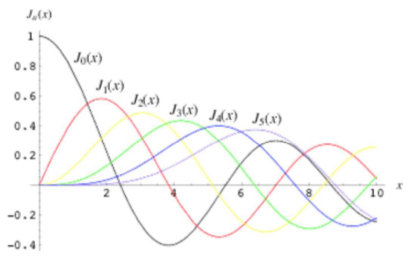
\includegraphics[scale=0.4]{ch6/image6}
	\captionof{figure}{ }
	\end{wrapfigure}
On peut faire apparaître les nouvelles harmoniques en développant la série de Fourier de \eqref{eq:6.38}
\begin{equation}
T = \frac{1}{2}+J_1\left(\pi\dfrac{V_m}{V_\pi}\right)\sin\omega_mt + J_3\left(\pi\dfrac{V_m}{V_\pi}\right)
\sin 3\omega_mt+ \dots
\end{equation}
où $J_i$ sont les fonctions de \textsc{Bessel}. Il semblerait au vue de la précédente expression que 
la bande passante soit infinie. L'amplitude des fonction de \textsc{Bessel} décroît cependant 
rapidement avec l'ordre. Si
\begin{equation}
\pi\dfrac{V_m}{V_\pi} <1
\end{equation}
Toutes les harmoniques sont négligeables et le signal de sortie est une réplique linéaire du signal de
modulation. Si ce n'est pas le cas, le signal de sortie présentera des distorsions.

\newpage
\subsection{Modulation en phase}
\iffalse



\fi






















